\documentclass{beamer}
\usetheme{Intel}

\setbeamertemplate{section in toc}{\inserttocsectionnumber.~\inserttocsection} % Use number keys for table of content sections.
\setbeamertemplate{subsection in toc}{\hspace{0.5cm}\rule[0.3ex]{3pt}{3pt}~\inserttocsubsection\par} % Use a symbol for table of content subsections.
\AtBeginSection[]
{
	\begin{frame}
		\frametitle{Table of Contents}
		\begin{multicols}{2}
			\tableofcontents[currentsection]
		\end{multicols}
    \end{frame}
} % Insert table of contents frame before each new section.
\setbeamertemplate{caption}[numbered] % Number figures.

\definecolor{intel}{RGB}{0, 113, 197}
\setbeamercolor{section in toc shaded}{fg=intel}
\setbeamercolor{subsection in toc shaded}{fg=black}
\setbeamercolor{section in toc}{fg=intel}
\setbeamercolor{subsection in toc}{fg=black}
\setbeamercolor{block title}{fg=intel}
\setbeamercolor{caption name}{fg=intel}

\usepackage{hyperref}
\usepackage{multicol} % Used to split up table of contents in a double column style.
\usepackage{multirow} % Needed for multirow graphs
\usepackage{datetime} % Used to format dates.
\usepackage{listings} % Used to format inline code throughout document.
\usepackage{color} % Used to gray out text
\usepackage{tikz} % Used to gain access to the \centering command.
\usepackage[mediumspace,mediumqspace,squaren,binary]{SIunits} % \milli\second

\hypersetup{
	colorlinks=false,
	linkcolor=blue,
	urlcolor=black,
	citecolor=blue,
	anchorcolor=blue
}
\usetikzlibrary{calc}

\newenvironment{graytext}{\color{gray}}{\ignorespacesafterend}

\newcommand{\mascfirstline}[1]{\input{#1}\unskip}

\lstset{
	language=C,
	tabsize=4,
	backgroundcolor=\color{black!5},
	basicstyle=\tiny,
}

\newcommand{\dvtcmdcodeinline}[1]{
	\colorbox{black!5}{
			\lstinline[basicstyle=\ttfamily\color{black}]{#1}}}

\newtheorem{thm}{Key point}

\begin{document}
	\title{Paravirtualizing OpenGL ES in Simics}
\subtitle{Master's Thesis in Computer Science}
\author{Eric Nilsson}
\institute{Intel Corporation}
\date{\today}

\begin{frame}
	\titlepage
\end{frame}


	\section{Introduction}

	\subsection{Simics}
	\begin{frame}

\frametitle{Wind River\texttrademark\ Simics\texttrademark }

\begin{itemize}
	\item Full-system simulator\note{That is; a fast and functional simulator that runs unmodified software}
	\item Originally devised at SICS\footnote{The Swedish Institute of Computer Science.}\note{This was the first instance of an unmodifed OS running in an entirely simulated environment}
	\item Developed by Intel\textregistered 
	\item Sold through Intels subsidiary Wind River Systems, Inc.
	\item Used in the industry by groups such as:
	\begin{itemize}
		\item IBM
		\item NASA
		\item Lockheed Martin
	\end{itemize}
	\item Utilized extensively in academia\footnote{$300+$ universities.}
\end{itemize}

\end{frame}


	\subsection{Key points}
	\begin{frame}
\frametitle{Question formulation}

\begin{block}{\#1}
  Is paravirtualization is a viable method of accelerating graphics?
\end{block}

\begin{block}{\#2}
  Are magic instructions is a suitable communications medium?
\end{block}

\begin{block}{\#3}
  How does hardware-assisted virtualization impact graphics acceleration using paravirtualization?
\end{block}

\end{frame}


        \subsection{Background}
        \begin{frame}
\frametitle{Background}

\begin{itemize}
\item Virtual platforms are key to reducing Time-to-Market
\item Improved simulation performance enables more use-cases
\item Because of architectural differences, GPU workloads are sub-optimal for CPUs
\item Therefore, some method of accelerating graphics in Simics is desireable
\end{itemize}

\begin{center}
{\Huge $\hookleftarrow$}
\end{center}

\end{frame}


	\subsection{Graphics simulation}
	\begin{frame}
\frametitle{Graphics simulation}

\begin{columns}
	\column{0.5\textwidth}
	\begin{block}{GPU modeling}
		Modeling the GPU ISA
                \begin{itemize}
                  \item Costly
                  \item Performance obstacles
                \end{itemize}
	\end{block}
	\begin{block}{PCI passthrough}
		First-hand device access using passthrough technologies
                \begin{itemize}
                  \item Requires dedicated hardware\phantom{     }
                  \item Difficult to implement robust checkpointing
                \end{itemize}
	\end{block}
    \column{0.5\textwidth}
    \begin{block}{Soft modeling}
    	Software rasterization
        \begin{itemize}
        \item Easy but often good-enough
        \item Performance obstacles
        \end{itemize}
    \end{block}
    \begin{block}{Paravirtualization}
    	Selectively modify virtual architecture
        \begin{itemize}
          \item Facilitate checkpointing in software
          \item Cost-effective but possibly heavy maintenence
        \end{itemize}
    \end{block}
\end{columns}
	
\end{frame}


        \section{Methodology and experiment}

        \subsection{Summary}
	\begin{frame}
  \frametitle{Summary}

  \begin{columns}
  \column{0.5\textwidth}

  \begin{block}{Method}
    \begin{itemize}
    \item Paravirtualized graphics
    \item Accelerates OpenGL ES 2.0
    \end{itemize}
  \end{block}

  \begin{block}{Evaluation}
    \begin{itemize}
    \item Run benchmarks stressing suspected optimal and sub-optimal use-case
    \item Compare performance to software rasterization
    \end{itemize}
  \end{block}

  \begin{block}{Conclusion}
    \begin{itemize}
    \item Improved performance, $34\times$
    \item Located bottleneck
    \end{itemize}
  \end{block}

  \column{0.5\textwidth}

  \begin{center}
    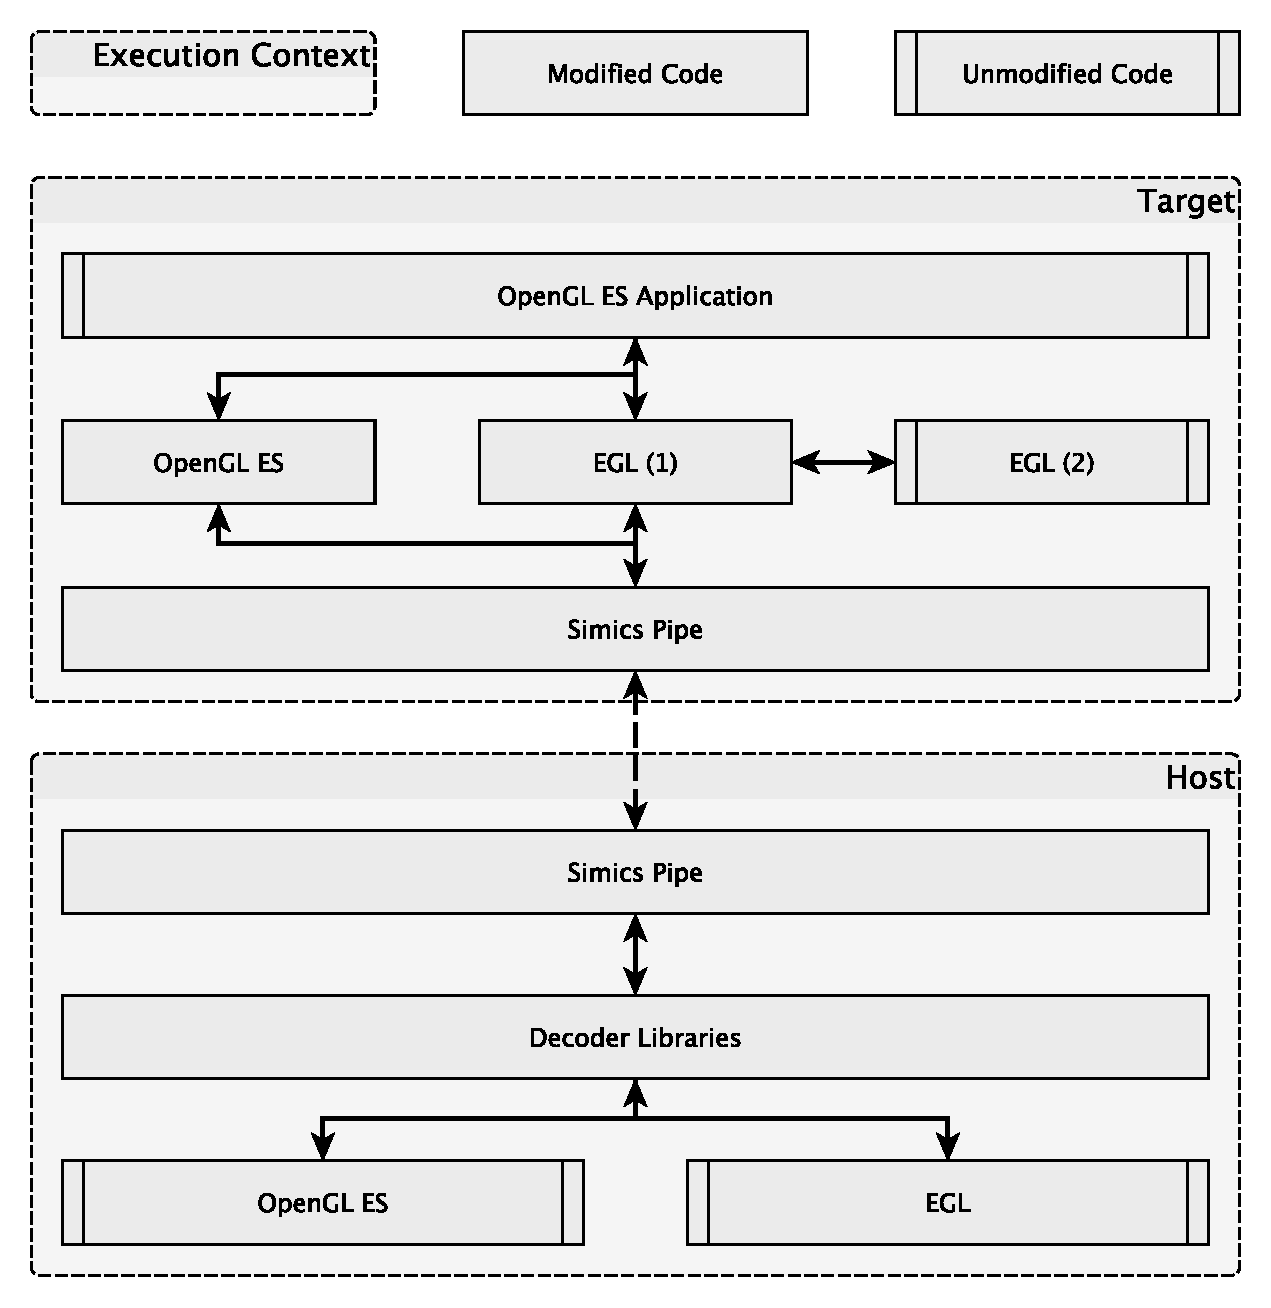
\includegraphics[height=0.7\textheight]{yedoverview.pdf}
  \end{center}

\end{columns}

\end{frame}


	\subsection{Simics pipe}
	\begin{frame}
\frametitle{Simics Pipe}

\begin{center}
	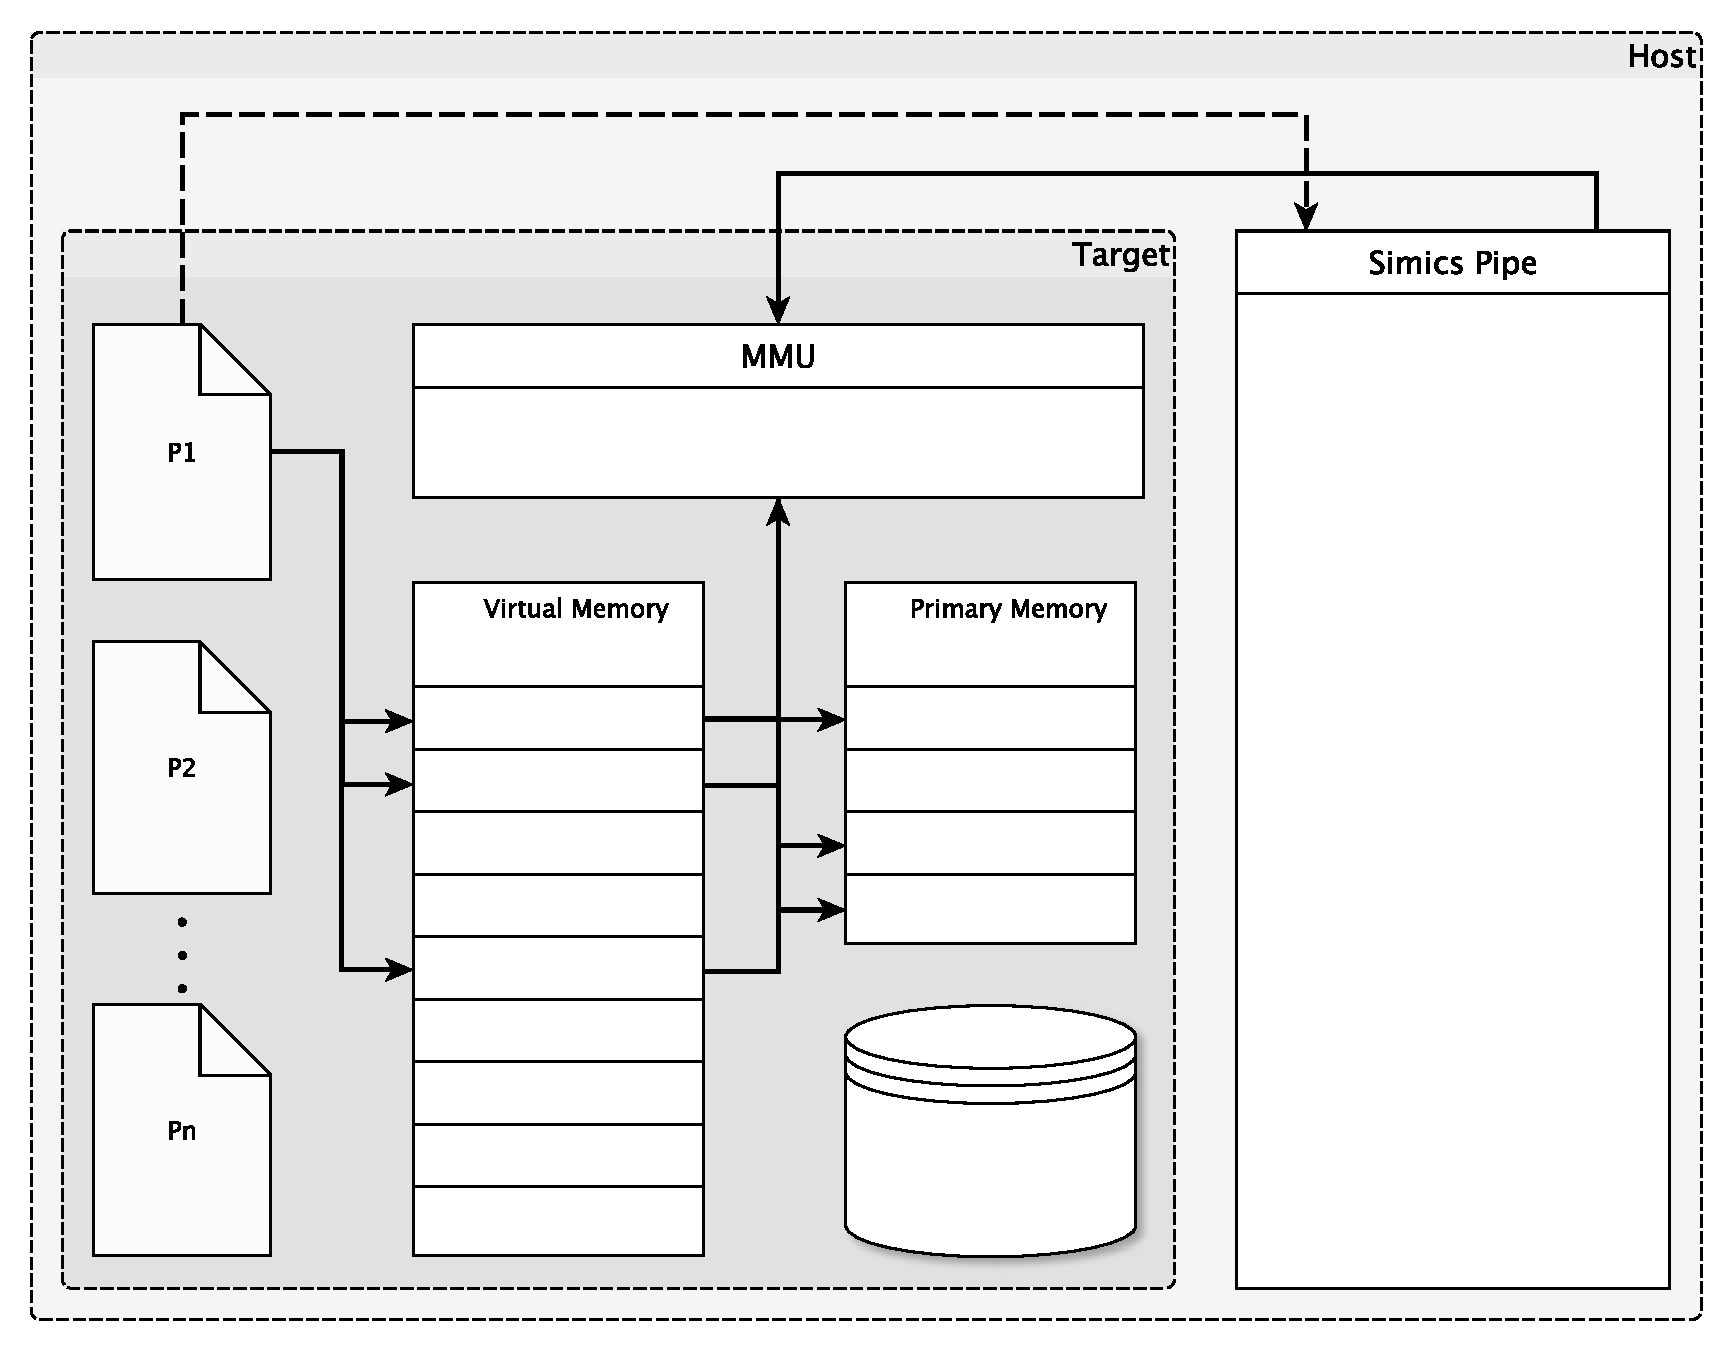
\includegraphics[height=0.8\textheight]{yedvirtualmemory.pdf}
\end{center}

\end{frame}

%% Memory translation overview. The OpenGL process hands a virtual memory
%% address, pointing somewhere in the target system \textit{primary}
%% memory, to the paravirtualized solution - which inquiries the target
%% system MMU to retrieve designated bytestream directly from target
%% physical memory.


        \subsection{Benchmarks}
	\begin{frame}[allowframebreaks]
\frametitle{Benchmarks}

%% % figbenchmarks.tex

\begin{figure}

\minipage{0.32\textwidth}
	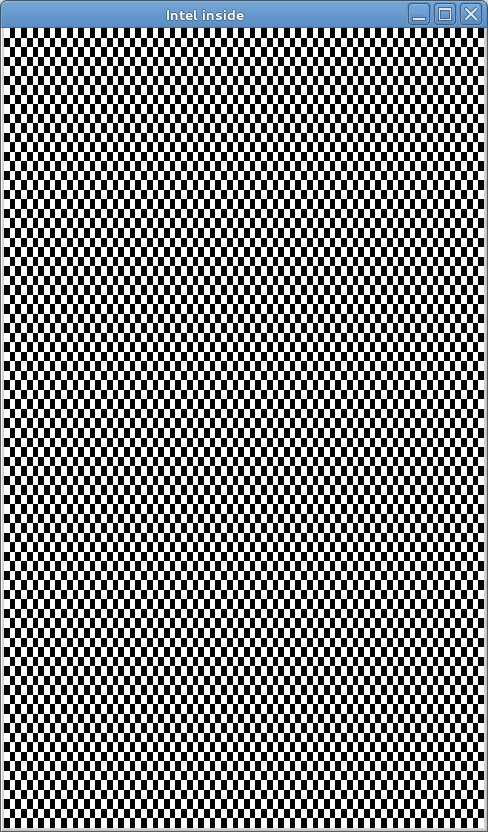
\includegraphics[width=\linewidth]{imgchess.png}
	\caption[Chess benchmark screen capture]{Chess.}
	\label{fig:benchmarks_chess}
\endminipage\hfill
\minipage{0.32\textwidth}
	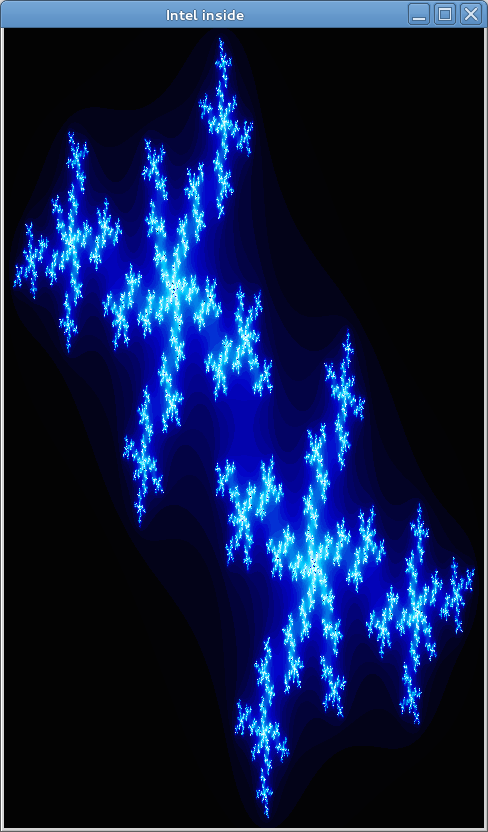
\includegraphics[width=\linewidth]{imgjulia.png}
	\caption[Julia benchmark screen capture]{Julia.}
	\label{fig:benchmarks_julia}
\endminipage\hfill
\minipage{0.32\textwidth}
  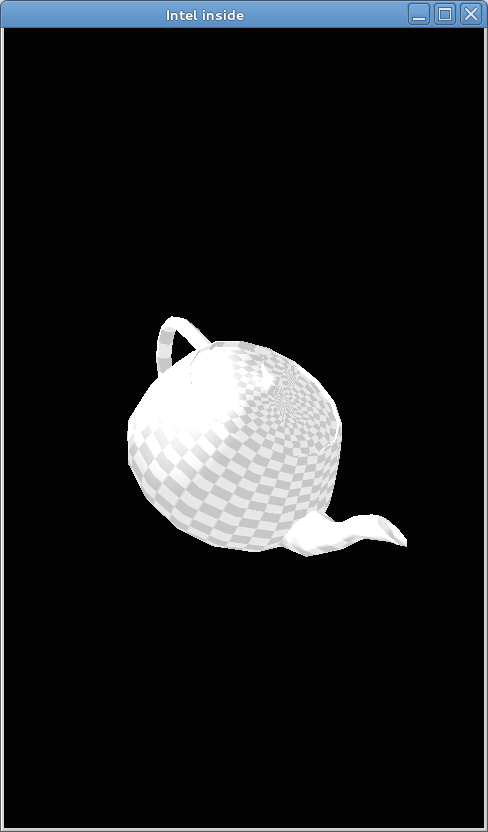
\includegraphics[width=\linewidth]{imgphong.png}
  \caption[Phong benchmark screen capture]{Phong.}
  \label{fig:benchmarks_phong}
\endminipage

\end{figure}

\framebreak 

%% \begin{block}{Input data variation}
%% \center
%% \resizebox{\linewidth}{!}{%
%% 	% tabkeyvals.tex

\begin{tabular}{lllll}
	Benchmark	& Input Data			& Halved Input		& Ref. Input		& Double Input		\\ \hline
	Chess		& No. Tiles				& $60\times60$		& $84\times84$		& $118\times118$	\\
	Julia		& No. Iterations		& $225$				& $450$				& $900$				\\
	Phong		& Texture Resolution	& $1448\times1448$	& $2048\times2048$	& $2896\times2896$	\\
\end{tabular}

%% }
%% \end{block}

%% \begin{block}{No. magic instructions}
%% \center
%% \resizebox{\linewidth}{!}{%
%% 	% tabkeyvalsmagicinstructions.tex

\begin{tabular}{lllll}
	Benchmark	& \phantom{Input Data}			& Halved Input	& Ref. Input	& Double Input	\\ \hline
	Chess		& \phantom{No. Tiles}			& $32403$		& $63507$		& $125319$		\\
	Julia		& \phantom{No. Iterations}		& $16$			& $16$			& $16$			\\
	Phong		& \phantom{Texture Resolution}	& $17$ 			& $17$ 			& $17$		\\
\end{tabular}

%% }
%% \end{block}
	
\end{frame}


        \subsection{Results}
        \providecommand{\chesskeyone}{$60\times60$ tiles}
\providecommand{\chesskeytwo}{$84\times84$ tiles}
\providecommand{\chesskeythree}{$118\times118$ tiles}

\providecommand{\juliakeyone}{$225$ iterations}
\providecommand{\juliakeytwo}{$450$ iterations}
\providecommand{\juliakeythree}{$900$ iterations}

\begin{frame}
  \frametitle{Results}

\end{frame}

        
	\section{Methodology}
	\subsection{Magic instructions}
	\begin{frame}
\frametitle{Magic instructions}

\begin{block}{Background}
	\begin{itemize}
		\item Many resons to escape simulation
		\begin{itemize}
			\item Breakpoints
			\item File sharing
			\item Profiling
		\end{itemize}
		\item Several methodologies
	\end{itemize}
\end{block}

\begin{block}{The 'Magic instruction'}
	\begin{itemize}
		\item \dvtcmdcodeinline{nop}-type instruction\footnotemark
		\item Potentially instant
		\item No modification to target system
	\end{itemize}
\end{block}

\footnotetext{\dvtcmdcodeinline{xchg ebx, ebx}}

\end{frame}


	\section{Experiment}

	\section{Results}
	\subsection{Histograms}
	\begin{frame}
\frametitle{Histograms}

\begin{center}
\resizebox{0.8\textwidth}{!}{%
	\input{gnuhistogramssimicsparachess.tex}
}
\end{center}

\begin{center}
\resizebox{0.8\textwidth}{!}{%
	\input{gnuhistogramssimicsparajulia.tex}
}
\end{center}

\end{frame}

	\subsection{Magic instruction overhead}
	% presentationmagicinstructionoverhead.tex

\begin{frame}[fragile]
\frametitle{Magic instruction overhead}
%% \begin{figure}
%% \centering
%% \begin{lstlisting}
%% int sercon = open("/dev/ttyS0",O_RDWR|O_NOCTTY);
%% \end{lstlisting}
%% \begin{minipage}{.5\textwidth}
%% 	\centering
	
%% \lstinputlisting{pseudoindividual.txt}
%% \end{minipage}%
%% \begin{minipage}{.5\textwidth}
%% 	\centering

%% \lstinputlisting{pseudobatch.txt}
%% \end{minipage}
%% \end{figure}

%% \begin{center}
%% % tabmagicinstructionsforall.tex

\begin{tabular}{llll}
Min & Max & Std & Avg \\ \hline
\dvtcmdfirstline{magicinstrprofileall.dat.min} & \dvtcmdfirstline{magicinstrprofileall.dat.max} & \dvtcmdfirstline{magicinstrprofileall.dat.std} & \dvtcmdfirstline{magicinstrprofileall.dat.avg} \\
\end{tabular}

%% \end{center}

\end{frame}


	\section{Discussion}
	\subsection{Deterministic execution}
	\begin{frame}

\frametitle{Deterministic execution}

Host dependency may affect simulation determinism\footnote{Variance affects only cross-platform simulation (checkpoints)}:
\begin{itemize}
	\item Hardware GPU floating point accuracy\footnote{Less of an issue since commonplace double floating point precision (2007)}
	\item Software API conformance (specification not necessarily strict)
\end{itemize}

However:
\begin{itemize}
	\item Often not an issue since graphics are commonly used only to display data
	\item Yet, GPU utilization for general purpose workloads increasingly more common
\end{itemize}

\textbf{Example}

\end{frame}

	\subsection{Checkpointing}
	\begin{frame}

\frametitle{Checkpointing}

\begin{block}{Conditions}
	\begin{itemize}
		\item Requires efficient framework functionality to store and restore system states (contestant:\dvtcmdcodeinline{glGet})
		\item Volatility; probable to be platform dependant in terms of efficiency
	\end{itemize}
\end{block}

\begin{block}{Related Work}
	Has been implemented in QEMU for OpenGL (Lagar-Cavilla et al.)
\end{block}

\begin{block}{Future Work}
	\begin{itemize}
		\item Transaction transparency in modern frameworks may advance the Checkpoint/Restart scheme in virtual platforms
		\item Experimental checkpoint schemes have been developed for CUDA (Guo et al.)
	\end{itemize}
\end{block}

\end{frame}

	\subsection{Reverse execution}
	\begin{frame}

\frametitle{Reverse execution}

\begin{block}{Currently}
	Graphics displayed exclusively in the host system
\end{block}

\begin{block}{Assumption}
	A potential productification of paravirtualized graphics would feature graphics output in the target system
\end{block}

\begin{block}{Prediction}
	\begin{itemize}
		\item If so, framebuffers would be present in target memory
		\item It follows that reverse execution functionality in Simics tracks said memory in checkpoints; effectively accomodating for reverse execution graphics
	\end{itemize}
\end{block}

\end{frame}


	\section{Conclusion}
	\subsection{Demonstration}
	\begin{frame}	

\frametitle{Demonstration}

\begin{block}{Julia Benchmark}
	\begin{itemize}
		\item \href{http://youtube.com/embed/GKs6OlWKFV8?rel=0&vq=hd1080&autoplay=1}{[Hardware accelerated on the simulation host]}
		\item \href{http://youtube.com/embed/3sCyzppFL0w?rel=0&vq=hd1080&autoplay=1}{[Software rasterized on the simulation target]}
		\item \href{http://youtube.com/embed/__d_EeZBzwc?rel=0&vq=hd1080&autoplay=1}{[Paravirtualized on the simulation target]}
	\end{itemize}
\end{block}

\end{frame}

	\subsection{Future work}
	\begin{frame}

\frametitle{Future work}

\begin{itemize}
  \item Command serialization batching \begin{itemize}\item WireGL\end{itemize}
  \item Extending supported frameworks \begin{itemize}\item DirectX $\rightarrow$ OpenGL\end{itemize}
  \item General purpose, GPGPU \begin{itemize}\item OpenCL\end{itemize}
\end{itemize}

\end{frame}

	\subsection{Key points recap}
	\begin{frame}
\frametitle{Question formulation}

\begin{block}{\#1}
  Is paravirtualization is a viable method of accelerating graphics?
\end{block}

\begin{block}{\#2}
  Are magic instructions is a suitable communications medium?
\end{block}

\begin{block}{\#3}
  How does hardware-assisted virtualization impact graphics acceleration using paravirtualization?
\end{block}

\end{frame}

\end{document}
